\documentclass{article}

\usepackage{arxiv}

\usepackage[utf8]{inputenc} % allow utf-8 input
\usepackage[T1]{fontenc}    % use 8-bit T1 fonts
\usepackage{lmodern}        % https://github.com/rstudio/rticles/issues/343
\usepackage{hyperref}       % hyperlinks
\usepackage{url}            % simple URL typesetting
\usepackage{booktabs}       % professional-quality tables
\usepackage{amsfonts}       % blackboard math symbols
\usepackage{nicefrac}       % compact symbols for 1/2, etc.
\usepackage{microtype}      % microtypography
\usepackage{graphicx}

\title{Assessing the influence of dopamine on the formation of
contextually appropriate visual routines}

\author{
    Kelly G. Garner
   \\
    School of Psychology \\
    University of New South Wales \\
  Sydney, NSW \\
  \texttt{\href{mailto:insert.unsw@here.edu.au}{\nolinkurl{insert.unsw@here.edu.au}}} \\
   \And
    Li-Ann Leow
   \\
    School of Psychology \\
    The University of Queensland \\
  St.~Lucia, QLD \\
  \texttt{} \\
   \And
    Aya Uchida
   \\
    School of Psychology \\
    The University of Queensland \\
  St.~Lucia, QLD \\
  \texttt{} \\
   \And
    Ole Jensen
   \\
    Center for Human Brain Health \\
    University of Birmingham \\
  Birmingham, UK \\
  \texttt{} \\
   \And
    Marta Garrido
   \\
    School of Psychological Sciences \\
    University of Melbourne \\
  Melbourne, VIC \\
  \texttt{} \\
   \And
    Paul E. Dux
   \\
    School of Psychology \\
    The University of Queensland \\
  St.~Lucia, QLD \\
  \texttt{} \\
  }


% tightlist command for lists without linebreak
\providecommand{\tightlist}{%
  \setlength{\itemsep}{0pt}\setlength{\parskip}{0pt}}

% From pandoc table feature
\usepackage{longtable,booktabs,array}
\usepackage{calc} % for calculating minipage widths
% Correct order of tables after \paragraph or \subparagraph
\usepackage{etoolbox}
\makeatletter
\patchcmd\longtable{\par}{\if@noskipsec\mbox{}\fi\par}{}{}
\makeatother
% Allow footnotes in longtable head/foot
\IfFileExists{footnotehyper.sty}{\usepackage{footnotehyper}}{\usepackage{footnote}}
\makesavenoteenv{longtable}

% Pandoc citation processing
\newlength{\cslhangindent}
\setlength{\cslhangindent}{1.5em}
\newlength{\csllabelwidth}
\setlength{\csllabelwidth}{3em}
\newlength{\cslentryspacingunit} % times entry-spacing
\setlength{\cslentryspacingunit}{\parskip}
% for Pandoc 2.8 to 2.10.1
\newenvironment{cslreferences}%
  {}%
  {\par}
% For Pandoc 2.11+
\newenvironment{CSLReferences}[2] % #1 hanging-ident, #2 entry spacing
 {% don't indent paragraphs
  \setlength{\parindent}{0pt}
  % turn on hanging indent if param 1 is 1
  \ifodd #1
  \let\oldpar\par
  \def\par{\hangindent=\cslhangindent\oldpar}
  \fi
  % set entry spacing
  \setlength{\parskip}{#2\cslentryspacingunit}
 }%
 {}
\usepackage{calc}
\newcommand{\CSLBlock}[1]{#1\hfill\break}
\newcommand{\CSLLeftMargin}[1]{\parbox[t]{\csllabelwidth}{#1}}
\newcommand{\CSLRightInline}[1]{\parbox[t]{\linewidth - \csllabelwidth}{#1}\break}
\newcommand{\CSLIndent}[1]{\hspace{\cslhangindent}#1}

\begin{document}
\maketitle


\begin{abstract}
Enter the text of your abstract here.
\end{abstract}

\keywords{
    blah
   \and
    blee
   \and
    bloo
   \and
    these are optional and can be removed
  }

\hypertarget{introduction}{%
\section{Introduction}\label{introduction}}

Here goes an introduction text

\hypertarget{methods}{%
\section{Methods}\label{methods}}

\label{sec:Methods}

\hypertarget{participants}{%
\subsection{Participants}\label{participants}}

A total of 40 participants (mean age: 24.5, sd: 5, 30 female, 10 male)
were recruited using the undergraduate and paid SONA pools administered
by the University of Queensland. All procedures were cleared by the
University of Queensland Human Research ethics committee
{[}2017/HE000847{]}, and were conducted in accordance with the National
Statement on Ethical Conduct in Human Research. Participants were over
18 years old, had no known neurological and psychiatric conditions
(assessed by self report), and no contraindications to Levodopa, as
assessed by the Levodopa safety screening questionnaire. Informed
consent was obtained at the start of the first session.

\hypertarget{procedure}{%
\subsection{Procedure}\label{procedure}}

Participants attended two sessions, spaced approximately 1 week apart.
After initial blood pressure and mood assessments, participants received
either placebo (vitamin C) or Levodopa (Madopar 125: 100 mg Levodopa and
25 mg Benserazide Hydrochloride), crushed and dispersed in orange juice,
now referred to as the `off' and `DA' sessions respectively. The
solution was prepared by an experimenter who did not administer the
remaining experimental procedures. This protocol was sufficient to
achieve double blinding in previous work
(\textbf{chowdhuryDopamineModulatesEpisodic2012?};
\textbf{chowdhuryDopamineRestoresReward2013?}). Participants then
completed the Five Facet Mindfulness Questionnaire
(\textbf{baerUsingSelfReportAssessment2006?}) and the Barratt
Impulsivity Scale {[}BIS;
(\textbf{pattonFactorStructureBarratt1995?}){]}, as trait impulsivity
scores are associated with midbrain dopamine D2/D3 receptor
availability. Around 30 minutes after drug administration, participants
completed a second blood pressure and mood rating assessment.
Participants then completed the practice stage of the task, so that the
experimental stage began approximately 40 minutes after drug ingestion,
within the window of peak plasma availability. At the end of the
session, participants completed the final blood pressure and mood rating
assessment and were asked whether they thought they had been given the
active or placebo drug.

\hypertarget{apparatus}{%
\subsection{Apparatus}\label{apparatus}}

The experimental task was run with custom code\footnote{\url{https://github.com/kel-github/variability-decision-making}},
written using Matlab 2012b (32 bit) and Psychtoolbox v3.0.14, on a
Windows 7 (64-bit) on a Dell Precision T1700 desktop computer, displayed
using a ASUS VG248 monitor. Gaze coordinates (x, y) were sampled at 120
Hz using a monitor-mounted iView Red-m infrared eye tracker
(SensoMotoric Instruments GmbH, Teltow, Germany). Participants were
seated from the monitor at an approximate viewing distance of 57 cm, and
positioned on a chin-rest for the duration of the task.

\hypertarget{experimental-task}{%
\subsection{Experimental Task}\label{experimental-task}}

Each trial began with a fixation dot presented centrally on a grey
screen {[}RGB: 200 200 200{]}. Participants were instructed to fixate on
the dot to begin a trial. After 1000 ms of continuous correct fixation
samples (within 100 pixels of fixation), a square was presented that
comprised 18° of degree visual angle from top to bottom (and
horizontally). The square could be one of four possible colours {[}RGBs:
87, 208, 169; 267, 145, 52; 167, 162, 229; 239, 91, 158{]}. After 1000
ms, a 4 x 4 grid of smaller squares appeared within the larger square,
in a darker version of the background colour ({[}RGB{]}-50). Each square
comprised 2.6° of visual angle. Participants were instructed that the 4
x 4 grid represented doors, and that they were to use their eyes to open
the doors to find where the target was hiding. Participants were also
instructed that they were to fixate on a single door to open it. When
participants had fixated on a single door for over 300 ms, the door
either turned black {[}RGB: 50, 50, 50{]}, to denote the absence of a
target, or the target was displayed and the trial was terminated. If the
door had turned black, it returned to its previous colour as soon as it
was detected that the participant had moved their eyes from the door.
Targets were animal images drawn randomly on each trial from a pool of
100 images taken from the internet. The time at which the target was
available to be found varied from trial to trial, with the onset being
drawn from a uniform distribution between 500-2000 ms. Once the target
was available and the correct door selected, the target was displayed
for 750 ms. Upon termination of the trial, the grey screen and white
fixation cross were presented (Fig 1A).

In each session, participants were shown two possible background and
door colour sets. Participants were instructed that each colour
represented a world, and that the animals had different places they
preferred to hide, depending on the world they were in. There were four
possible target locations within each world, or from here on, context.
For each context, 1 door from each quadrant was selected as a potential
target location (see Fig 1B), and target locations could not overlap
between contexts. Thus each colour reflected a context in which
participants could establish a set of goal relevant eye-movements,
i.e.~towards the 4 possible target locations for that context. Note that
within each context, the target was equally likely to appear behind any
one of the 4 target doors (p=.25) and would never appear behind the
remaining doors (p=0). Colour-target location mappings were
counterbalanced across participants, as was the assignment of coloured
contexts to sessions. Participants completed 80 trials in each context.
Eye-movement calibration and validation was performed every 20 trials.
Participants were also shown the standard QWERTY keyboard and were
instructed that they could press `x' at any time to perform a new
calibration and validation if they felt that their eye-movements were no
longer being registered accurately; i.e.~if they were unable to open
doors even though they were selecting them.

\begin{figure}

{\centering 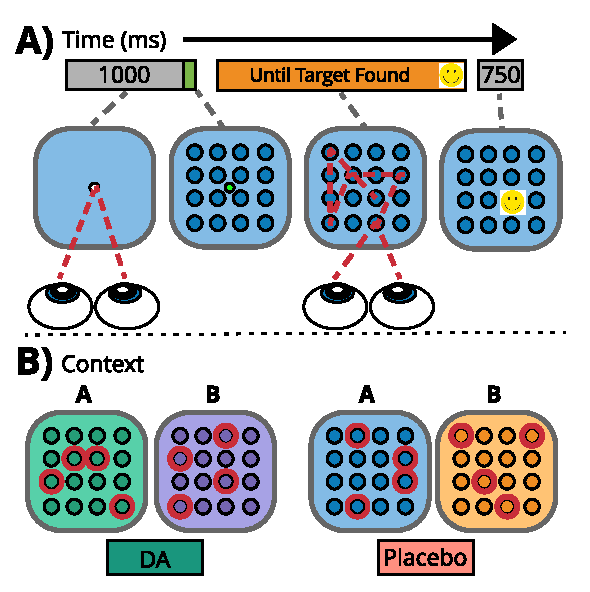
\includegraphics[width=0.7\linewidth]{../../images/DA_ExpTask} 

}

\caption{Experimental Task. A) A single trial where participants use their eyes to open doors to locate a target. B) Contexts and sessions: in each session, participants are exposed to two colour contexts each with 4 unique and equiprobable target locations. In each session, Levodopa or placebo is administered under double blind conditions.}\label{fig:taskfig}
\end{figure}

\hypertarget{statistical-approach}{%
\subsection{Statistical Approach}\label{statistical-approach}}

The analysis was designed to assess the learning of the target locations
given the context, the extent to which eye-movements became
stereotypical, and how both of these measures were modulated by the
dopamine and mindfulness factors.

\hypertarget{data-cleaning}{%
\subsubsection{Data cleaning}\label{data-cleaning}}

Doors were marked as selected if participants gazed at them for a
duration of at least 300 ms. We assumed that a door could not be
selected twice consecutively, and collapsed any consecutive duplications
into a single door selection. Last, as the final door selection of every
trial was fixed (i.e.~finding the target location ends trial), we
removed the final selection from each trial for the sequence analysis
defined below. We excluded data from one participant whose total number
of door selections was greater than 3 standard deviations from the mean
across both sessions. The remaining 39 datasets were retained for all of
the analyses. Note that this is more inclusive than our pre-registered
plan for data exclusions\footnote{\url{https://osf.io/2y6pk}}. Based on
pilot data, we had planned to exclude participants who scored
\textless{} 65\% accuracy over the course of a session. However,
analysis of the final sample suggested that this was too stringent, as
this resulted in the exclusion of 23/40 participants.

\hypertarget{accuracy-data}{%
\subsection{Accuracy data}\label{accuracy-data}}

We sought to determine the extent to which participants learned the
target locations, and whether participants learned to select the doors
that were relevant given the current context. Door selections were
classified as target relevant (TR) for the current context (cc), the
other context from that session (oc), or neither (n). Data was then
grouped into blocks of 10 trials per context, and grouped across
contexts, resulting in 8 blocks of 20 trials. First, to determine
whether participants learned the target locations overall, we counted
the number of correct door selections (referred to from now as accuracy
{[}acc{]}):

\[
acc = \sum{(TR_{cc}, TR_{oc})}
\]

To assess the influence of block and drug (DA vs off) on accuracy, we
fit Bayesian mixed effects models with the following general form:

NOTE: NEED TO WORK OUT HOW TO GET THIS ONTO SEPARATE LINES

\[
acc_{i} \sim Bin(n_{i}, p_{i}) \\
logit(p_{i}) = \mu_{i} \\
\mu_{i}|x_{i}, \beta, z_{i}, b_{i} \sim \mathcal{N}(X_{i}\beta + Z_{i}b_{i}, \sigma^2) \\
i = 1, ... N \\
\]

where \(i\) = 1 to N participants. X is a matrix containing fixed effect
regressors for block, and drug (DA vs.~off), and any interactions. Z is
a matrix of random effects regressors including subject intercepts and
slopes, containing regressors for the block and drug effects and their
interaction. \(\mathcal{N}\) is a normal distribution with standard
deviation \(\sigma^2\). \(n_{i}\) is the total number of door selections
(cc + oc + n), and \(p_{i}\) is the probability of attaining \(acc_{i}\)
given \(n_{i}\).

For this and following analyses, we sought to find the model that best
fit the data, and then made inference over the resulting parameters.
Models were fit using the BRMS
(\textbf{burknerBrmsPackageBayesian2017?}) interface for Stan
(\textbf{standevelopmentteamStanModelingLanguage?}) and RStan
(\textbf{standevelopmentteamRStanInterfaceStan2023?}) in R
(\textbf{rcoreteamLanguageEnvironmentStatistical2015?}). We used the
default weakly informative priors as specified in
(\textbf{burknerBrmsPackageBayesian2017?}). Specifically, \(\beta\) and
\(b\) coefficients were given a flat prior, intercept and standard
deviations were assumed to be drawn from a student's \(t\) distribution
(df=1, location=0, scale=2.5), and the LKJ-correlation prior with
parameter \(\zeta\) \textgreater{} 0 was used for the parameter
covariance matrix.

To find the best fitting model, we fit models containing each
combination of the block and drug regressors (and associated random
effects), and found the best model using leave-one-out (LOO) cross
validation (as implemented in
\textbf{vehtariPracticalBayesianModel2017?}). (Note that in the
pre-registration document we had proposed to compare models using the
deviance information criterion (DIC). As, LOO is more robust than DIC to
influential observations, and is readily implemented for use with BRMS
model objects, we opted to use LOO instead of DIC). Upon identifying the
best model from the experimentally manipulated regressors, we then added
the mindfulness regressor in all possible combinations with the best
model, until increasing complexity provided no further gains in
prediction (as evidenced by LOO). Last we controlled for trait
impulsivity by adding BIS scores as a regressor to the winning model. In
all cases, we sought to use the most complex random effects structure as
is supported by the data (\textbf{barrRandomEffectsStructure2013?}).
Note that even though we used model selection, the inference over
parameters was consistent across models.

\hypertarget{contextual-accuracy}{%
\subsection{Contextual Accuracy}\label{contextual-accuracy}}

We also sought to understand whether dopamine modulates the ability of
participants to select the correct door, given the context. Therefore,
for each context, we computed the total number of cc door selections
(c-acc), and modelled the probability of attaining c-acc given the total
number of correct door selections (i.e.~\(n_{i}\) from equation X
becomes \(\sum (TR_{cc}, TR_{oc}\)).

We then fit this data with Bayesian mixed effects models following the
procedure above (Note that in the pre-registration document we had
suggested to include a regressor for context. Visual inspection of the
data showed that c-acc was highly comparable across contexts {[}see
supplemental figures{]}. We therefore opted to eschew a larger parameter
space and collapsed over this factor).

\hypertarget{stereotypical-sequences}{%
\subsection{Stereotypical sequences}\label{stereotypical-sequences}}

Next, we seek to determine whether eye-movement patterns become more
stereotypical over the course of the task, and whether dopamine and
mindfulness modulates the extent of stereotypy. Here we define
stereotypy as sets of door selections being deployed in the same order,
over trials. Therefore we wish to know whether, given the set of doors
that a participant chose to open over the trials of the experiment, did
they select them in a particular order more than would be expected by
chance?

In order to characterise the extent to which the order of door
selections differed from what would be expected by chance, we computed a
null hypothesis for each subject, generated under the assumption that
there is no temporal regularity in their door selection patterns. This
null hypothesis was then used as a regressor in a hierarchical model
that we describe below. If additional parameters are required to account
for the data over and above the theoretical null regressor, then those
parameters are interpreted as implying the presence and extent of
stereotypy, modulated by the experimental factor coded by the additional
parameter.

The construction of the null hypothesis is as follows: to identify how a
participant's data should look under the null, we take the door
selections from any given trial, and given those selections, we compute
all the possible permutations of door selection order, excluding any
permutation where the same door is selected twice consecutively. For any
given set of trials, we then compute the transition matrix; given that
the participant is in the state of being at door x, how many times did
they move to door y? The resulting transition matrix forms the null
hypothesis for that subject, which can be compared to the observed
transition counts for that subject and set of trials. Note that we
present simulation results demonstrating the suitability of this method
in our pre-registration document\footnote{\url{https://osf.io/xn6d2/}}.

The observed transition counts were using the same model structure as
defined above, with the addition of the null regressor. Identification
of the best random effects structure and the winning model proceeded as
described for the accuracy data above. Mindfulness and impulsivity
scores were added to the winning model, again according to the procedure
outlined above.

\hypertarget{control-analyses}{%
\subsection{Control analyses}\label{control-analyses}}

To determine whether awareness of the dopamine intervention could have
contributed to the findings, the probability of participant and
experimenter ratings will be compared to the expected values assuming
chance guessing, using a binomial model. Blood-pressure and mood
measures were compared using {[}insert whether paired t-test or
Mann-Whitney U test{]}.

LaTeX command can be used to reference other section. See Section
\ref{sec:headings}. However, you can also use \textbf{bookdown}
extensions mechanism for this.

\hypertarget{headings-second-level}{%
\subsection{Headings: second level}\label{headings-second-level}}

You can use equation in blocks

\[
\xi _{ij}(t)=P(x_{t}=i,x_{t+1}=j|y,v,w;\theta)= {\frac {\alpha _{i}(t)a^{w_t}_{ij}\beta _{j}(t+1)b^{v_{t+1}}_{j}(y_{t+1})}{\sum _{i=1}^{N} \sum _{j=1}^{N} \alpha _{i}(t)a^{w_t}_{ij}\beta _{j}(t+1)b^{v_{t+1}}_{j}(y_{t+1})}}
\]

But also inline i.e \(z=x+y\)

\hypertarget{headings-third-level}{%
\subsubsection{Headings: third level}\label{headings-third-level}}

Another paragraph.

\hypertarget{examples-of-citations-figures-tables-references}{%
\section{Examples of citations, figures, tables,
references}\label{examples-of-citations-figures-tables-references}}

\label{sec:others}

You can insert references. Here is some text (Kour and Saabne 2014b,
2014a) and see Hadash et al. (2018).

The documentation for \verb+natbib+ may be found at

You can use custom blocks with LaTeX support from \textbf{rmarkdown} to
create environment.

\begin{center}
\url{http://mirrors.ctan.org/macros/latex/contrib/natbib/natnotes.pdf\%7D}

\end{center}

Of note is the command \verb+\citet+, which produces citations
appropriate for use in inline text.

You can insert LaTeX environment directly too.

\begin{verbatim}
   \citet{hasselmo} investigated\dots
\end{verbatim}

produces

\begin{quote}
  Hasselmo, et al.\ (1995) investigated\dots
\end{quote}

\begin{center}
  \url{https://www.ctan.org/pkg/booktabs}
\end{center}

\hypertarget{figures}{%
\subsection{Figures}\label{figures}}

You can insert figure using LaTeX directly.

See Figure \ref{fig:fig1}. Here is how you add footnotes. {[}\^{}Sample
of the first footnote.{]}

\begin{figure}
  \centering
  \fbox{\rule[-.5cm]{4cm}{4cm} \rule[-.5cm]{4cm}{0cm}}
  \caption{Sample figure caption.}
  \label{fig:fig1}
\end{figure}

But you can also do that using R.

\begin{figure}

{\centering 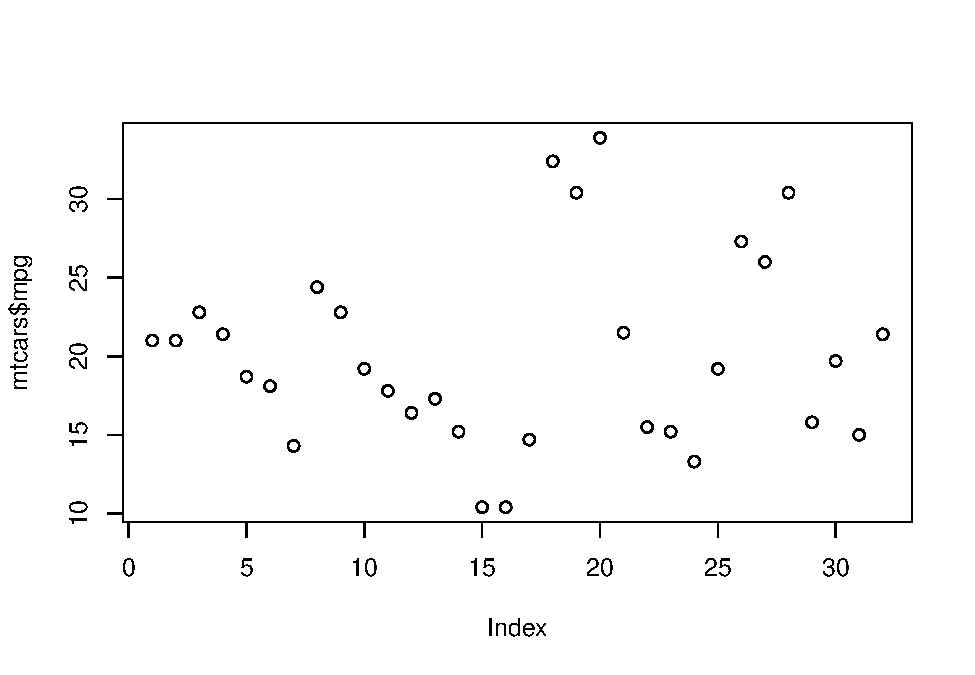
\includegraphics{assessing-the-role-of-dopamine-on-the-formation-of-contextually-relevant-visual-routines_files/figure-latex/fig2-1} 

}

\caption{Another sample figure}\label{fig:fig2}
\end{figure}

You can use \textbf{bookdown} to allow references for Tables and
Figures.

\hypertarget{tables}{%
\subsection{Tables}\label{tables}}

Below we can see how to use tables.

See awesome Table\textasciitilde{}\ref{tab:table} which is written
directly in LaTeX in source Rmd file.

\begin{table}
 \caption{Sample table title}
  \centering
  \begin{tabular}{lll}
    \toprule
    \multicolumn{2}{c}{Part}                   \\
    \cmidrule(r){1-2}
    Name     & Description     & Size ($\mu$m) \\
    \midrule
    Dendrite & Input terminal  & $\sim$100     \\
    Axon     & Output terminal & $\sim$10      \\
    Soma     & Cell body       & up to $10^6$  \\
    \bottomrule
  \end{tabular}
  \label{tab:table}
\end{table}

You can also use R code for that.

\begin{longtable}[]{@{}
  >{\raggedright\arraybackslash}p{(\columnwidth - 22\tabcolsep) * \real{0.2687}}
  >{\raggedleft\arraybackslash}p{(\columnwidth - 22\tabcolsep) * \real{0.0746}}
  >{\raggedleft\arraybackslash}p{(\columnwidth - 22\tabcolsep) * \real{0.0597}}
  >{\raggedleft\arraybackslash}p{(\columnwidth - 22\tabcolsep) * \real{0.0746}}
  >{\raggedleft\arraybackslash}p{(\columnwidth - 22\tabcolsep) * \real{0.0597}}
  >{\raggedleft\arraybackslash}p{(\columnwidth - 22\tabcolsep) * \real{0.0746}}
  >{\raggedleft\arraybackslash}p{(\columnwidth - 22\tabcolsep) * \real{0.0746}}
  >{\raggedleft\arraybackslash}p{(\columnwidth - 22\tabcolsep) * \real{0.0746}}
  >{\raggedleft\arraybackslash}p{(\columnwidth - 22\tabcolsep) * \real{0.0448}}
  >{\raggedleft\arraybackslash}p{(\columnwidth - 22\tabcolsep) * \real{0.0448}}
  >{\raggedleft\arraybackslash}p{(\columnwidth - 22\tabcolsep) * \real{0.0746}}
  >{\raggedleft\arraybackslash}p{(\columnwidth - 22\tabcolsep) * \real{0.0746}}@{}}
\caption{Head of mtcars table}\tabularnewline
\toprule()
\begin{minipage}[b]{\linewidth}\raggedright
\end{minipage} & \begin{minipage}[b]{\linewidth}\raggedleft
mpg
\end{minipage} & \begin{minipage}[b]{\linewidth}\raggedleft
cyl
\end{minipage} & \begin{minipage}[b]{\linewidth}\raggedleft
disp
\end{minipage} & \begin{minipage}[b]{\linewidth}\raggedleft
hp
\end{minipage} & \begin{minipage}[b]{\linewidth}\raggedleft
drat
\end{minipage} & \begin{minipage}[b]{\linewidth}\raggedleft
wt
\end{minipage} & \begin{minipage}[b]{\linewidth}\raggedleft
qsec
\end{minipage} & \begin{minipage}[b]{\linewidth}\raggedleft
vs
\end{minipage} & \begin{minipage}[b]{\linewidth}\raggedleft
am
\end{minipage} & \begin{minipage}[b]{\linewidth}\raggedleft
gear
\end{minipage} & \begin{minipage}[b]{\linewidth}\raggedleft
carb
\end{minipage} \\
\midrule()
\endfirsthead
\toprule()
\begin{minipage}[b]{\linewidth}\raggedright
\end{minipage} & \begin{minipage}[b]{\linewidth}\raggedleft
mpg
\end{minipage} & \begin{minipage}[b]{\linewidth}\raggedleft
cyl
\end{minipage} & \begin{minipage}[b]{\linewidth}\raggedleft
disp
\end{minipage} & \begin{minipage}[b]{\linewidth}\raggedleft
hp
\end{minipage} & \begin{minipage}[b]{\linewidth}\raggedleft
drat
\end{minipage} & \begin{minipage}[b]{\linewidth}\raggedleft
wt
\end{minipage} & \begin{minipage}[b]{\linewidth}\raggedleft
qsec
\end{minipage} & \begin{minipage}[b]{\linewidth}\raggedleft
vs
\end{minipage} & \begin{minipage}[b]{\linewidth}\raggedleft
am
\end{minipage} & \begin{minipage}[b]{\linewidth}\raggedleft
gear
\end{minipage} & \begin{minipage}[b]{\linewidth}\raggedleft
carb
\end{minipage} \\
\midrule()
\endhead
Mazda RX4 & 21.0 & 6 & 160 & 110 & 3.90 & 2.62 & 16.5 & 0 & 1 & 4 & 4 \\
Mazda RX4 Wag & 21.0 & 6 & 160 & 110 & 3.90 & 2.88 & 17.0 & 0 & 1 & 4 &
4 \\
Datsun 710 & 22.8 & 4 & 108 & 93 & 3.85 & 2.32 & 18.6 & 1 & 1 & 4 & 1 \\
Hornet 4 Drive & 21.4 & 6 & 258 & 110 & 3.08 & 3.21 & 19.4 & 1 & 0 & 3 &
1 \\
Hornet Sportabout & 18.7 & 8 & 360 & 175 & 3.15 & 3.44 & 17.0 & 0 & 0 &
3 & 2 \\
Valiant & 18.1 & 6 & 225 & 105 & 2.76 & 3.46 & 20.2 & 1 & 0 & 3 & 1 \\
\bottomrule()
\end{longtable}

\hypertarget{lists}{%
\subsection{Lists}\label{lists}}

\begin{itemize}
\tightlist
\item
  Item 1
\item
  Item 2
\item
  Item 3
\end{itemize}

\hypertarget{refs}{}
\begin{CSLReferences}{1}{0}
\leavevmode\vadjust pre{\hypertarget{ref-hadash2018estimate}{}}%
Hadash, Guy, Einat Kermany, Boaz Carmeli, Ofer Lavi, George Kour, and
Alon Jacovi. 2018. {``Estimate and Replace: A Novel Approach to
Integrating Deep Neural Networks with Existing Applications.''}
\emph{arXiv Preprint arXiv:1804.09028}.

\leavevmode\vadjust pre{\hypertarget{ref-kour2014fast}{}}%
Kour, George, and Raid Saabne. 2014a. {``Fast Classification of
Handwritten on-Line Arabic Characters.''} In \emph{Soft Computing and
Pattern Recognition (SoCPaR), 2014 6th International Conference of},
312--18. IEEE.

\leavevmode\vadjust pre{\hypertarget{ref-kour2014real}{}}%
---------. 2014b. {``Real-Time Segmentation of on-Line Handwritten
Arabic Script.''} In \emph{Frontiers in Handwriting Recognition (ICFHR),
2014 14th International Conference on}, 417--22. IEEE.

\end{CSLReferences}

\bibliographystyle{unsrt}
\bibliography{references.bib}


\end{document}
